本システムは、取引成立時の手数料収益を核に、取引量の増加とマッチング精度の向上が相互に促進し合う「データ駆動の改善サイクル」を中核に据えた事業モデルを採用する。図\ref{fig:business}に、主要ステークホルダー間の価値の流れと、データ蓄積・学習・改善の循環構造を示す。

\begin{figure}[htbp]
\centering
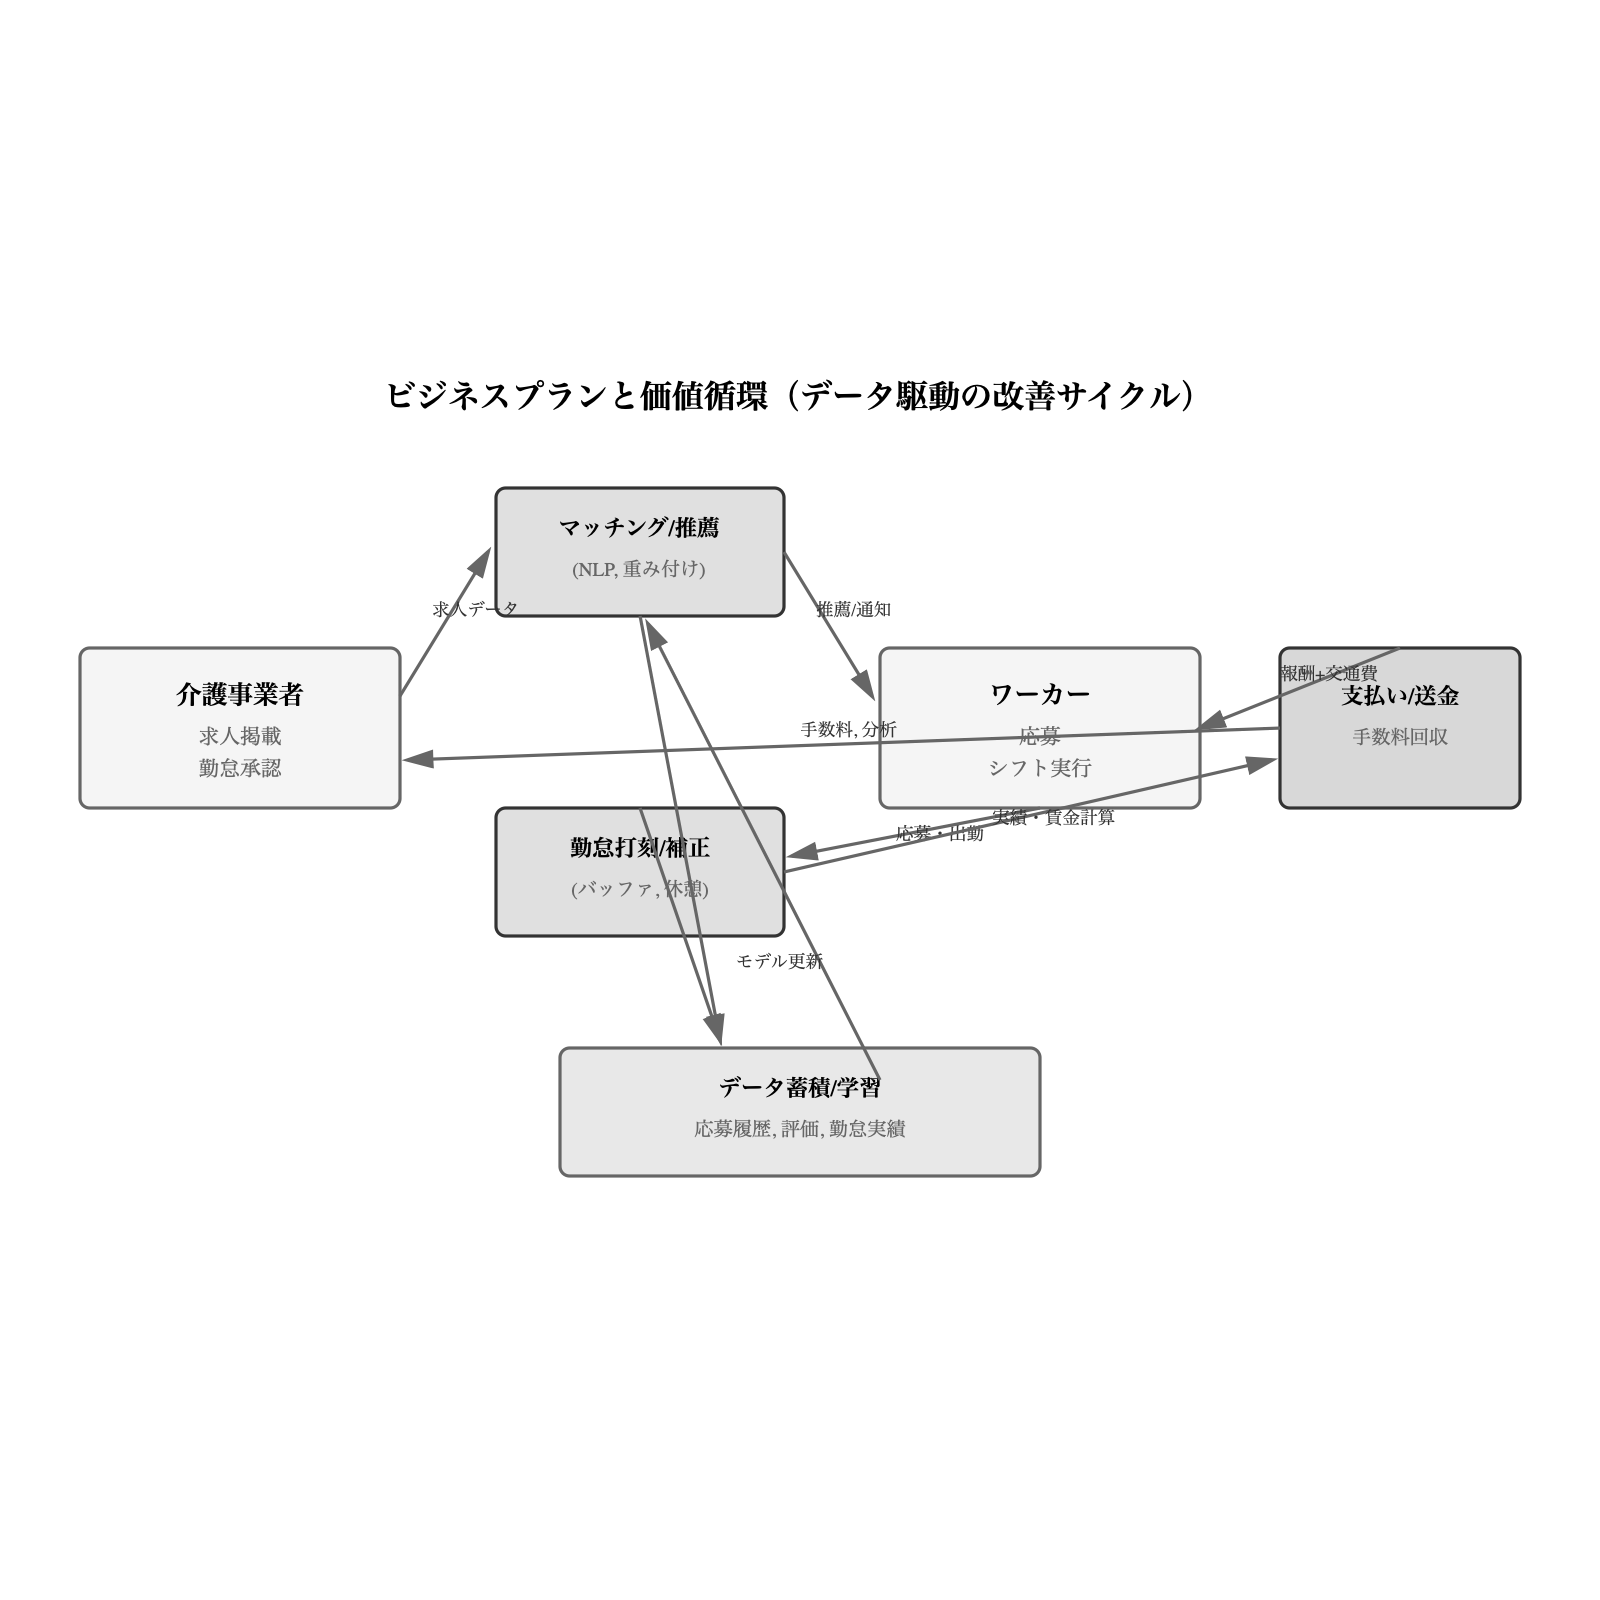
\includegraphics[width=0.95\textwidth]{images/fig1-8.png}
\caption{ビジネスプランと価値循環（データ駆動の改善サイクル）}
\label{fig:business}
\end{figure}

価値循環のメカニズムは以下の通りである。（1）\textbf{求人掲載から応募へ}：事業者が掲載した求人情報は、NLPモデルによる意味的類似性計算と過去の履歴分析に基づき、適合度の高いワーカーに推薦される。（2）\textbf{応募から勤務実行へ}：ワーカーの応募・採用・勤怠打刻の一連のデータが蓄積され、どの求人条件が実際の就業に結びつきやすいかが分析される。（3）\textbf{支払いと手数料回収}：勤務実績に基づく賃金計算と送金が自動化され、プラットフォームは手数料を回収する。この収益は、アルゴリズム改善やシステム拡張への投資原資となる。（4）\textbf{データ学習とモデル更新}：蓄積された応募履歴、勤怠実績、評価データから、マッチング推薦モデルが継続的に学習・更新される。精度が向上すればワーカーの満足度と定着率が高まり、事業者の採用効率も改善する。結果として取引量が増加し、さらに多様なデータが蓄積されるという正のフィードバックが形成される。このサイクルにより、初期投資を回収しつつ長期的に持続可能な事業成長が可能となる。なお、本研究はこの「データ学習とモデル更新」の部分に焦点を当て、学習方法や更新方針の改善を目指す。
